\documentclass{article}
\usepackage{tikz}
\usetikzlibrary{arrows.meta,positioning,shapes.geometric}
\usepackage[margin=0.3in]{geometry}
\pagestyle{empty}

\begin{document}

% Title
\begin{center}
\textbf{\Large Circular Buffer Architecture - Packet Flow Timeline}\\
\vspace{2mm}
\textit{12KB Ring Buffer with Strict FIFO Order}
\end{center}

\vspace{5mm}

% ============================================================================
% STATE 1: T=0ms - Initial State (3 packets in buffer)
% ============================================================================
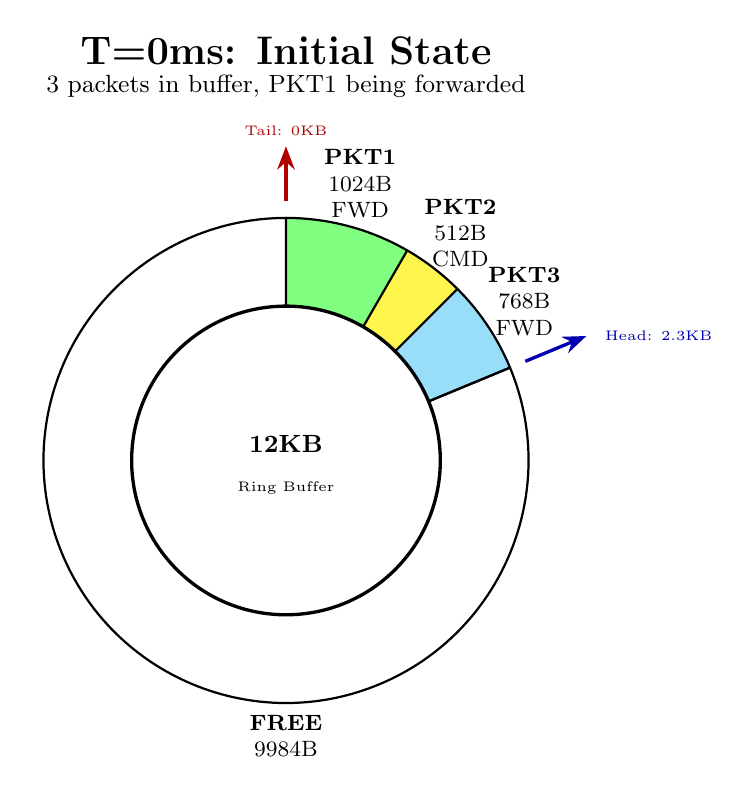
\begin{tikzpicture}[>=Stealth,font=\sffamily,semithick,scale=1.4]

    % State label
    \node [above,font=\Large\bfseries] at (0,3.5) {T=0ms: Initial State};
    \node [above,font=\small] at (0,3.2) {3 packets in buffer, PKT1 being forwarded};

    % PKT1 (90° to 60°): Forward packet - GREEN
    \fill [green!50] (0,0) -- (90:2.2) arc [start angle=90, end angle=60, radius=2.2] -- cycle;
    \draw [thick] (90:2.2) arc [start angle=90, end angle=60, radius=2.2];
    \node [align=center,font=\footnotesize] at (75:2.6) {\textbf{PKT1}\\1024B\\FWD};

    % PKT2 (60° to 45°): Command packet - YELLOW
    \fill [yellow!70] (0,0) -- (60:2.2) arc [start angle=60, end angle=45, radius=2.2] -- cycle;
    \draw [thick] (60:2.2) arc [start angle=60, end angle=45, radius=2.2];
    \node [align=center,font=\footnotesize] at (52.5:2.6) {\textbf{PKT2}\\512B\\CMD};

    % PKT3 (45° to 22.5°): Forward packet - CYAN
    \fill [cyan!40] (0,0) -- (45:2.2) arc [start angle=45, end angle=22.5, radius=2.2] -- cycle;
    \draw [thick] (45:2.2) arc [start angle=45, end angle=22.5, radius=2.2];
    \node [align=center,font=\footnotesize] at (33.75:2.6) {\textbf{PKT3}\\768B\\FWD};

    % FREE SPACE
    \fill [white,draw=black,thick] (0,0) -- (22.5:2.2) arc [start angle=22.5, end angle=-270, radius=2.2] -- cycle;
    \node [align=center,font=\footnotesize] at (270:2.5) {\textbf{FREE}\\9984B};

    % Radial dividers
    \draw [thick] (0,0) -- (90:2.2);
    \draw [thick] (0,0) -- (60:2.2);
    \draw [thick] (0,0) -- (45:2.2);
    \draw [thick] (0,0) -- (22.5:2.2);

    % Inner circle
    \draw [very thick,fill=white] (0,0) circle (1.4);
    \node [align=center,font=\small\bfseries] at (0,0.15) {12KB};
    \node [align=center,font=\tiny] at (0,-0.25) {Ring Buffer};

    % Tail pointer
    \draw [->,very thick,red!70!black,line width=1.2pt] (90:2.35) -- (90:2.85)
        node [above,font=\tiny] {Tail: 0KB};

    % Head pointer
    \draw [->,very thick,blue!70!black,line width=1.2pt] (22.5:2.35) -- (22.5:2.95)
        node [right,xshift=1mm,font=\tiny] {Head: 2.3KB};

\end{tikzpicture}
\hspace{5mm}
% ============================================================================
% STATE 2: T=2.3ms - PKT1 Released
% ============================================================================
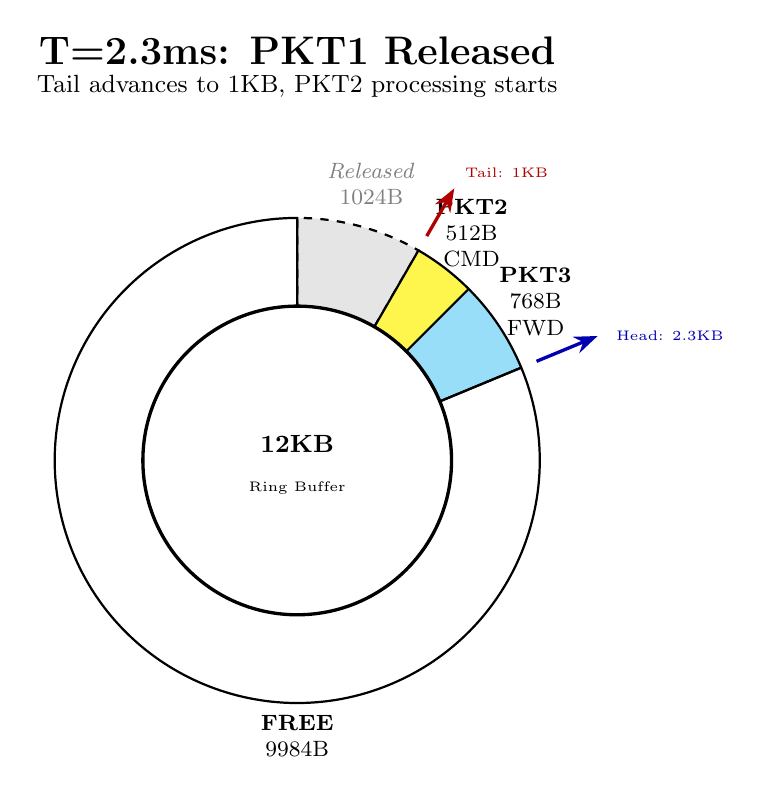
\begin{tikzpicture}[>=Stealth,font=\sffamily,semithick,scale=1.4]

    % State label
    \node [above,font=\Large\bfseries] at (0,3.5) {T=2.3ms: PKT1 Released};
    \node [above,font=\small] at (0,3.2) {Tail advances to 1KB, PKT2 processing starts};

    % PKT1 RELEASED (shown as freed space)
    \fill [gray!20,draw=black,thick,dashed] (0,0) -- (90:2.2) arc [start angle=90, end angle=60, radius=2.2] -- cycle;
    \node [align=center,font=\footnotesize,text=gray] at (75:2.6) {\textit{Released}\\1024B};

    % PKT2 (60° to 45°): Command packet - YELLOW (now being processed)
    \fill [yellow!70] (0,0) -- (60:2.2) arc [start angle=60, end angle=45, radius=2.2] -- cycle;
    \draw [thick] (60:2.2) arc [start angle=60, end angle=45, radius=2.2];
    \node [align=center,font=\footnotesize] at (52.5:2.6) {\textbf{PKT2}\\512B\\CMD};

    % PKT3 (45° to 22.5°): Forward packet - CYAN (waiting)
    \fill [cyan!40] (0,0) -- (45:2.2) arc [start angle=45, end angle=22.5, radius=2.2] -- cycle;
    \draw [thick] (45:2.2) arc [start angle=45, end angle=22.5, radius=2.2];
    \node [align=center,font=\footnotesize] at (33.75:2.6) {\textbf{PKT3}\\768B\\FWD};

    % FREE SPACE (larger now)
    \fill [white,draw=black,thick] (0,0) -- (22.5:2.2) arc [start angle=22.5, end angle=-270, radius=2.2] -- cycle;
    \node [align=center,font=\footnotesize] at (270:2.5) {\textbf{FREE}\\9984B};

    % Radial dividers
    \draw [thick] (0,0) -- (90:2.2);
    \draw [thick] (0,0) -- (60:2.2);
    \draw [thick] (0,0) -- (45:2.2);
    \draw [thick] (0,0) -- (22.5:2.2);

    % Inner circle
    \draw [very thick,fill=white] (0,0) circle (1.4);
    \node [align=center,font=\small\bfseries] at (0,0.15) {12KB};
    \node [align=center,font=\tiny] at (0,-0.25) {Ring Buffer};

    % Tail pointer (MOVED to 60°)
    \draw [->,very thick,red!70!black,line width=1.2pt] (60:2.35) -- (60:2.85)
        node [above right,font=\tiny] {Tail: 1KB};

    % Head pointer (unchanged)
    \draw [->,very thick,blue!70!black,line width=1.2pt] (22.5:2.35) -- (22.5:2.95)
        node [right,xshift=1mm,font=\tiny] {Head: 2.3KB};

\end{tikzpicture}

\vspace{5mm}

% ============================================================================
% STATE 3: T=2.5ms - PKT2 Released
% ============================================================================
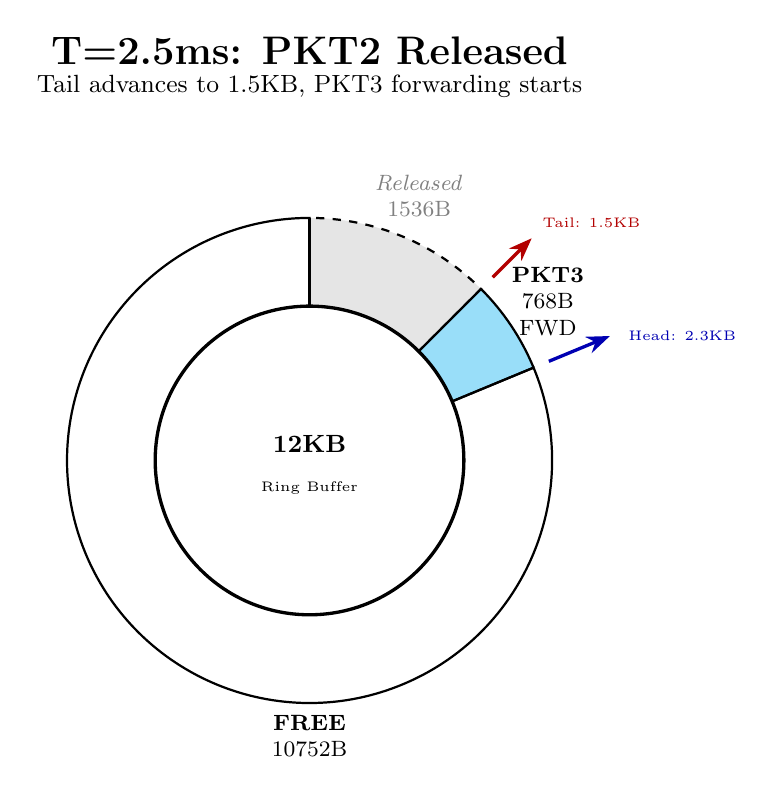
\begin{tikzpicture}[>=Stealth,font=\sffamily,semithick,scale=1.4]

    % State label
    \node [above,font=\Large\bfseries] at (0,3.5) {T=2.5ms: PKT2 Released};
    \node [above,font=\small] at (0,3.2) {Tail advances to 1.5KB, PKT3 forwarding starts};

    % PKT1 & PKT2 RELEASED
    \fill [gray!20,draw=black,thick,dashed] (0,0) -- (90:2.2) arc [start angle=90, end angle=45, radius=2.2] -- cycle;
    \node [align=center,font=\footnotesize,text=gray] at (67.5:2.6) {\textit{Released}\\1536B};

    % PKT3 (45° to 22.5°): Forward packet - CYAN (being forwarded)
    \fill [cyan!40] (0,0) -- (45:2.2) arc [start angle=45, end angle=22.5, radius=2.2] -- cycle;
    \draw [thick] (45:2.2) arc [start angle=45, end angle=22.5, radius=2.2];
    \node [align=center,font=\footnotesize] at (33.75:2.6) {\textbf{PKT3}\\768B\\FWD};

    % FREE SPACE (even larger)
    \fill [white,draw=black,thick] (0,0) -- (22.5:2.2) arc [start angle=22.5, end angle=-270, radius=2.2] -- cycle;
    \node [align=center,font=\footnotesize] at (270:2.5) {\textbf{FREE}\\10752B};

    % Radial dividers
    \draw [thick] (0,0) -- (90:2.2);
    \draw [thick] (0,0) -- (45:2.2);
    \draw [thick] (0,0) -- (22.5:2.2);

    % Inner circle
    \draw [very thick,fill=white] (0,0) circle (1.4);
    \node [align=center,font=\small\bfseries] at (0,0.15) {12KB};
    \node [align=center,font=\tiny] at (0,-0.25) {Ring Buffer};

    % Tail pointer (MOVED to 45°)
    \draw [->,very thick,red!70!black,line width=1.2pt] (45:2.35) -- (45:2.85)
        node [above right,font=\tiny] {Tail: 1.5KB};

    % Head pointer (unchanged)
    \draw [->,very thick,blue!70!black,line width=1.2pt] (22.5:2.35) -- (22.5:2.95)
        node [right,xshift=1mm,font=\tiny] {Head: 2.3KB};

\end{tikzpicture}
\hspace{5mm}
% ============================================================================
% STATE 4: T=5ms - New Packets Arrive
% ============================================================================
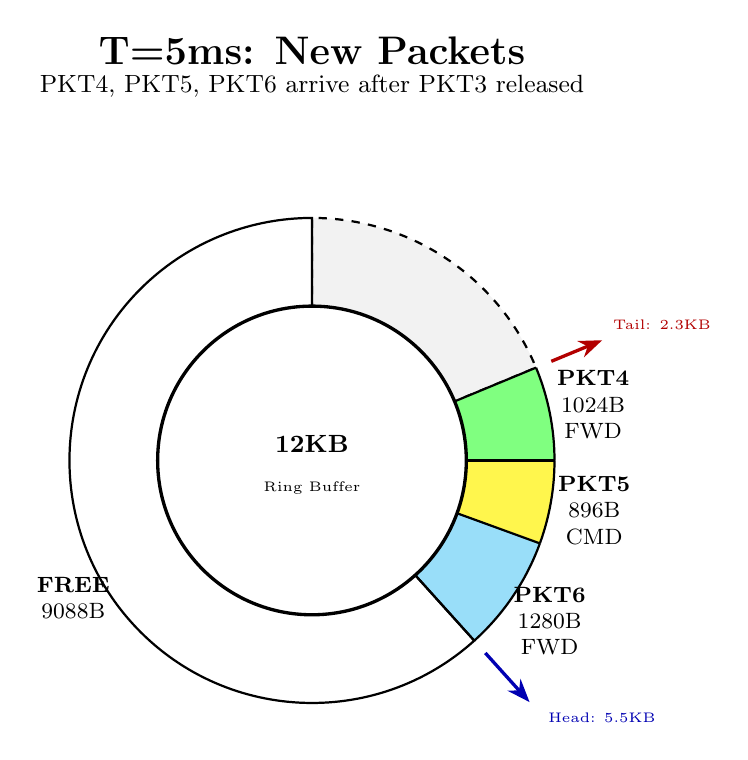
\begin{tikzpicture}[>=Stealth,font=\sffamily,semithick,scale=1.4]

    % State label
    \node [above,font=\Large\bfseries] at (0,3.5) {T=5ms: New Packets};
    \node [above,font=\small] at (0,3.2) {PKT4, PKT5, PKT6 arrive after PKT3 released};

    % All previous released (shown very lightly)
    \fill [gray!10,draw=black,thick,dashed] (0,0) -- (90:2.2) arc [start angle=90, end angle=22.5, radius=2.2] -- cycle;

    % PKT4 (22.5° to 0°): Forward packet - GREEN
    \fill [green!50] (0,0) -- (22.5:2.2) arc [start angle=22.5, end angle=0, radius=2.2] -- cycle;
    \draw [thick] (22.5:2.2) arc [start angle=22.5, end angle=0, radius=2.2];
    \node [align=center,font=\footnotesize] at (11.25:2.6) {\textbf{PKT4}\\1024B\\FWD};

    % PKT5 (0° to -20°): Command packet - YELLOW
    \fill [yellow!70] (0,0) -- (0:2.2) arc [start angle=0, end angle=-20, radius=2.2] -- cycle;
    \draw [thick] (0:2.2) arc [start angle=0, end angle=-20, radius=2.2];
    \node [align=center,font=\footnotesize] at (-10:2.6) {\textbf{PKT5}\\896B\\CMD};

    % PKT6 (-20° to -48°): Forward packet - CYAN
    \fill [cyan!40] (0,0) -- (-20:2.2) arc [start angle=-20, end angle=-48, radius=2.2] -- cycle;
    \draw [thick] (-20:2.2) arc [start angle=-20, end angle=-48, radius=2.2];
    \node [align=center,font=\footnotesize] at (-34:2.6) {\textbf{PKT6}\\1280B\\FWD};

    % FREE SPACE
    \fill [white,draw=black,thick] (0,0) -- (-48:2.2) arc [start angle=-48, end angle=-270, radius=2.2] -- cycle;
    \node [align=center,font=\footnotesize] at (210:2.5) {\textbf{FREE}\\9088B};

    % Radial dividers
    \draw [thick] (0,0) -- (22.5:2.2);
    \draw [thick] (0,0) -- (0:2.2);
    \draw [thick] (0,0) -- (-20:2.2);
    \draw [thick] (0,0) -- (-48:2.2);

    % Inner circle
    \draw [very thick,fill=white] (0,0) circle (1.4);
    \node [align=center,font=\small\bfseries] at (0,0.15) {12KB};
    \node [align=center,font=\tiny] at (0,-0.25) {Ring Buffer};

    % Tail pointer (back to 22.5° after wraparound)
    \draw [->,very thick,red!70!black,line width=1.2pt] (22.5:2.35) -- (22.5:2.85)
        node [above right,font=\tiny] {Tail: 2.3KB};

    % Head pointer (MOVED to -48°)
    \draw [->,very thick,blue!70!black,line width=1.2pt] (-48:2.35) -- (-48:2.95)
        node [below right,xshift=1mm,font=\tiny] {Head: 5.5KB};

\end{tikzpicture}

\vspace{5mm}

% ============================================================================
% STATE 5: Wraparound Scenario
% ============================================================================
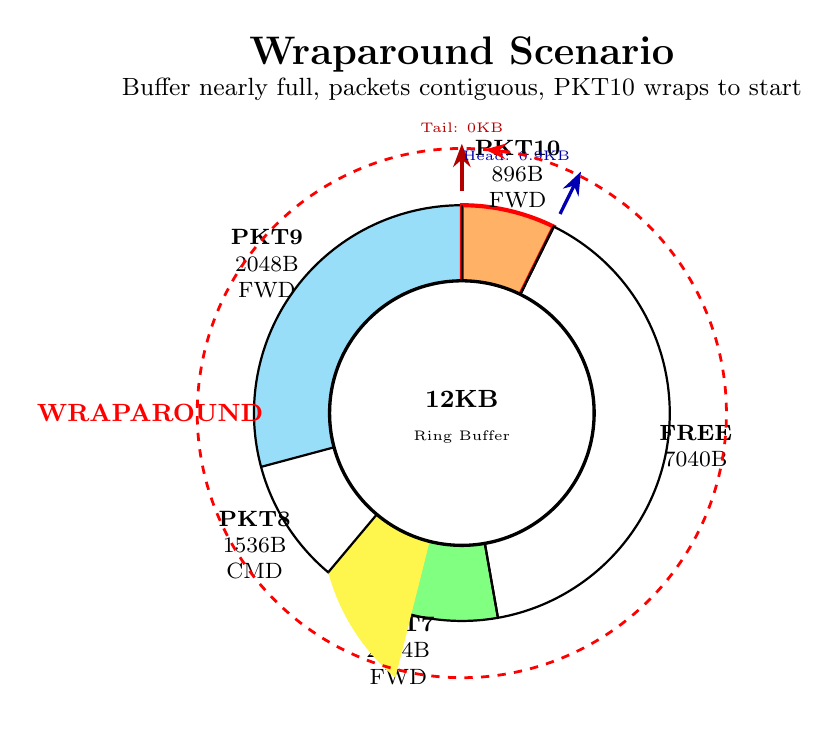
\begin{tikzpicture}[>=Stealth,font=\sffamily,semithick,scale=1.2]

    % State label
    \node [above,font=\Large\bfseries] at (0,3.5) {Wraparound Scenario};
    \node [above,font=\small] at (0,3.2) {Buffer nearly full, packets contiguous, PKT10 wraps to start};

    % PKT7 (-80° to -130°): Large forward packet
    \fill [green!50] (0,0) -- (-80:2.2) arc [start angle=-80, end angle=-130, radius=2.2] -- cycle;
    \draw [thick] (-80:2.2) arc [start angle=-80, end angle=-130, radius=2.2];
    \node [align=center,font=\footnotesize] at (-105:2.6) {\textbf{PKT7}\\2304B\\FWD};

    % PKT8 (-130° to -165°): Command
    \fill [yellow!70] (0,0) -- (-130:2.2) arc [start angle=-165, end angle=-130, radius=2.2] -- cycle;
    \draw [thick] (-130:2.2) arc [start angle=-130, end angle=-165, radius=2.2];
    \node [align=center,font=\footnotesize] at (-147.5:2.6) {\textbf{PKT8}\\1536B\\CMD};

    % PKT9 (-165° to -270°): Forward packet extends to buffer end (NO GAP)
    \fill [cyan!40] (0,0) -- (-165:2.2) arc [start angle=-165, end angle=-270, radius=2.2] -- cycle;
    \draw [thick] (-165:2.2) arc [start angle=-165, end angle=-270, radius=2.2];
    \node [align=center,font=\footnotesize] at (-217.5:2.6) {\textbf{PKT9}\\2048B\\FWD};

    % PKT10 wrapping (90° to 63.75°): Wraparound packet at buffer start - ORANGE with red border
    \fill [orange!60,draw=red,thick,line width=1.5pt] (0,0) -- (90:2.2) arc [start angle=90, end angle=63.75, radius=2.2] -- cycle;
    \node [align=center,font=\footnotesize] at (76.875:2.6) {\textbf{PKT10}\\896B\\FWD};

    % FREE SPACE - continuous region between head and tail (63.75° to -80°)
    \fill [white,draw=black,thick] (0,0) -- (63.75:2.2) arc [start angle=63.75, end angle=-80, radius=2.2] -- cycle;
    \node [align=center,font=\footnotesize] at (-8:2.5) {\textbf{FREE}\\7040B};

    % Radial dividers
    \draw [thick] (0,0) -- (90:2.2);
    \draw [thick] (0,0) -- (63.75:2.2);
    \draw [thick] (0,0) -- (-80:2.2);
    \draw [thick] (0,0) -- (-130:2.2);
    \draw [thick] (0,0) -- (-165:2.2);
    \draw [thick] (0,0) -- (-270:2.2);

    % Inner circle
    \draw [very thick,fill=white] (0,0) circle (1.4);
    \node [align=center,font=\small\bfseries] at (0,0.15) {12KB};
    \node [align=center,font=\tiny] at (0,-0.25) {Ring Buffer};

    % Tail pointer at buffer start
    \draw [->,very thick,red!70!black,line width=1.2pt] (90:2.35) -- (90:2.85)
        node [above,font=\tiny] {Tail: 0KB};

    % Head pointer after PKT10
    \draw [->,very thick,blue!70!black,line width=1.2pt] (63.75:2.35) -- (63.75:2.85)
        node [above left,font=\tiny] {Head: 0.9KB};

    % Wraparound annotation showing continuous allocation
    \draw [->,very thick,red,dashed,line width=1pt] (-280:2.8) arc [start angle=-280, end angle=85, radius=2.8];
    \node [red,font=\small\bfseries] at (180:3.3) {WRAPAROUND};

\end{tikzpicture}
\hspace{5mm}
% ============================================================================
% STATE 6: After PKT7 Released
% ============================================================================
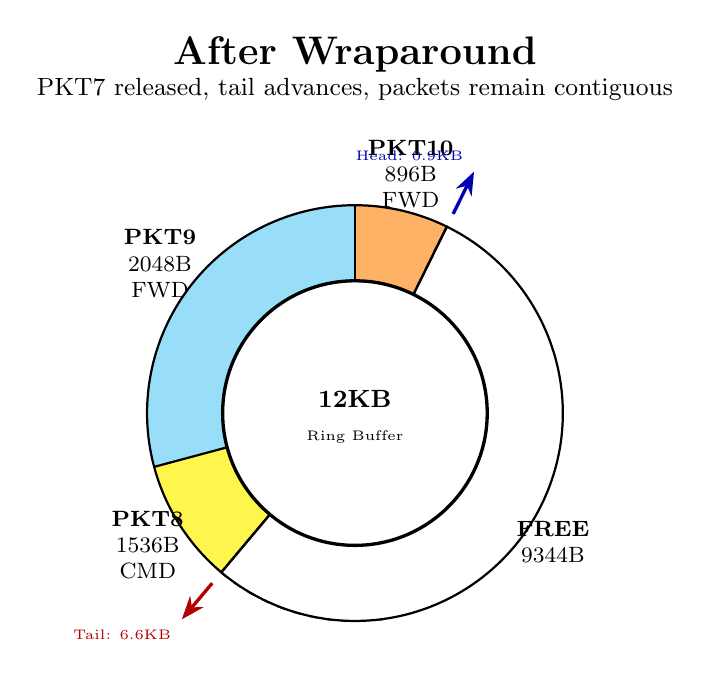
\begin{tikzpicture}[>=Stealth,font=\sffamily,semithick,scale=1.2]

    % State label
    \node [above,font=\Large\bfseries] at (0,3.5) {After Wraparound};
    \node [above,font=\small] at (0,3.2) {PKT7 released, tail advances, packets remain contiguous};

    % PKT7 RELEASED (shown in gray dashed)
    \fill [gray!20,draw=black,thick,dashed] (0,0) -- (-80:2.2) arc [start angle=-80, end angle=-130, radius=2.2] -- cycle;

    % PKT8 (-130° to -165°): Command (being processed)
    \fill [yellow!70] (0,0) -- (-130:2.2) arc [start angle=-130, end angle=-165, radius=2.2] -- cycle;
    \draw [thick] (-130:2.2) arc [start angle=-130, end angle=-165, radius=2.2];
    \node [align=center,font=\footnotesize] at (-147.5:2.6) {\textbf{PKT8}\\1536B\\CMD};

    % PKT9 (-165° to -270°): Forward packet extends to buffer end (contiguous)
    \fill [cyan!40] (0,0) -- (-165:2.2) arc [start angle=-165, end angle=-270, radius=2.2] -- cycle;
    \draw [thick] (-165:2.2) arc [start angle=-165, end angle=-270, radius=2.2];
    \node [align=center,font=\footnotesize] at (-217.5:2.6) {\textbf{PKT9}\\2048B\\FWD};

    % PKT10 (90° to 63.75°) at buffer start (wraparound position)
    \fill [orange!60] (0,0) -- (90:2.2) arc [start angle=90, end angle=63.75, radius=2.2] -- cycle;
    \draw [thick] (90:2.2) arc [start angle=90, end angle=63.75, radius=2.2];
    \node [align=center,font=\footnotesize] at (76.875:2.6) {\textbf{PKT10}\\896B\\FWD};

    % FREE SPACE - continuous region between head and tail (63.75° to -130°)
    \fill [white,draw=black,thick] (0,0) -- (63.75:2.2) arc [start angle=63.75, end angle=-130, radius=2.2] -- cycle;
    \node [align=center,font=\footnotesize] at (-33:2.5) {\textbf{FREE}\\9344B};

    % Radial dividers
    \draw [thick] (0,0) -- (90:2.2);
    \draw [thick] (0,0) -- (63.75:2.2);
    \draw [thick] (0,0) -- (-130:2.2);
    \draw [thick] (0,0) -- (-165:2.2);
    \draw [thick] (0,0) -- (-270:2.2);

    % Inner circle
    \draw [very thick,fill=white] (0,0) circle (1.4);
    \node [align=center,font=\small\bfseries] at (0,0.15) {12KB};
    \node [align=center,font=\tiny] at (0,-0.25) {Ring Buffer};

    % Tail pointer (MOVED to -130° after PKT7 released)
    \draw [->,very thick,red!70!black,line width=1.2pt] (-130:2.35) -- (-130:2.85)
        node [below left,font=\tiny] {Tail: 6.6KB};

    % Head pointer (unchanged at 63.75°)
    \draw [->,very thick,blue!70!black,line width=1.2pt] (63.75:2.35) -- (63.75:2.85)
        node [above left,font=\tiny] {Head: 0.9KB};

\end{tikzpicture}

\vspace{5mm}

% ============================================================================
% Legend and Summary
% ============================================================================
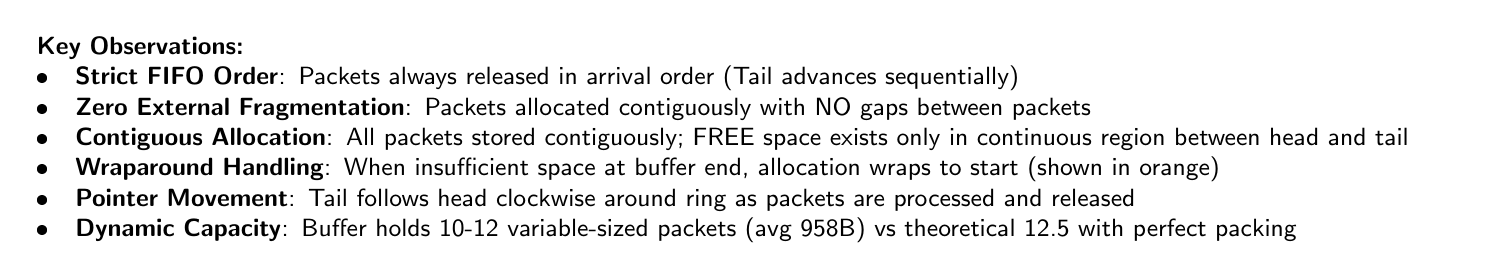
\begin{tikzpicture}[font=\sffamily\small]
    \node [align=left,text width=18cm] at (0,0) {
        \textbf{Key Observations:}\\
        \textbullet\quad \textbf{Strict FIFO Order}: Packets always released in arrival order (Tail advances sequentially)\\
        \textbullet\quad \textbf{Zero External Fragmentation}: Packets allocated contiguously with NO gaps between packets\\
        \textbullet\quad \textbf{Contiguous Allocation}: All packets stored contiguously; FREE space exists only in continuous region between head and tail\\
        \textbullet\quad \textbf{Wraparound Handling}: When insufficient space at buffer end, allocation wraps to start (shown in orange)\\
        \textbullet\quad \textbf{Pointer Movement}: Tail follows head clockwise around ring as packets are processed and released\\
        \textbullet\quad \textbf{Dynamic Capacity}: Buffer holds 10-12 variable-sized packets (avg 958B) vs theoretical 12.5 with perfect packing
    };
\end{tikzpicture}

\vspace{5mm}

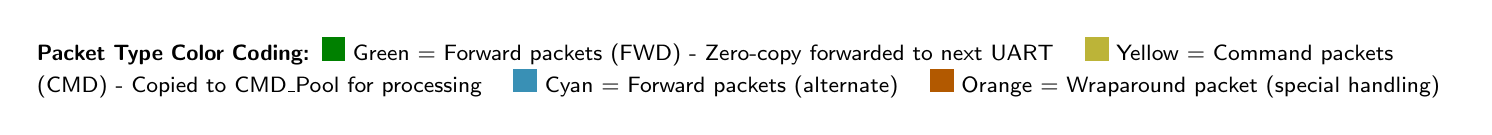
\begin{tikzpicture}[font=\sffamily\footnotesize]
    \node [align=left,text width=18cm] at (0,0) {
        \textbf{Packet Type Color Coding:}
        \textcolor{green!50!black}{\rule{3mm}{3mm}} Green = Forward packets (FWD) - Zero-copy forwarded to next UART \quad
        \textcolor{yellow!70!black}{\rule{3mm}{3mm}} Yellow = Command packets (CMD) - Copied to CMD\_Pool for processing \quad
        \textcolor{cyan!70!black}{\rule{3mm}{3mm}} Cyan = Forward packets (alternate) \quad
        \textcolor{orange!70!black}{\rule{3mm}{3mm}} Orange = Wraparound packet (special handling)
    };
\end{tikzpicture}

\end{document}
